\section{\textbf{Safe Boolean MRSW Register}}
% ------------------------------------------------------------------------------------ %
\subsection{Particular Case}
\par
In class we saw the difference between Safe, Regular and Atomic Registers. In
this excersice we are experimenting with a Safe Boolean Register. In particular,
we are trying a register that allows one single writer whose writen value can be
examined by multiple readers. We need to remember that Safe registers are those
that :
\begin{itemize}
\item If a read does not overlap with a write, then the read returns the last
written value
\item If a read overlaps with a write, then the read can return any value in the
domain of the register's values
\end{itemize}
% ------------------------------------------------------------------------------------ %
\subsection{Solution}
\par
One way to achive this behaviour is using a SRSW Safe register. The code that is
provided with the book does this by having a boolean SRSW register per thread,
in other words, it is an array of boolean values. When doing a write, the writer
iterates over this array and writes the new value. The readers simply access its
assigned slot in the array (based on the thread id) and return the stored value. 
% ------------------------------------------------------------------------------------ %
\subsection{Experiment Description}
\par
This program provides two test cases. The first one is a sequential test and the
second one is a parallel test. The former simply calls a write and then a read
from the same thread. This is not rocket science. The reader must retrieve what
the writer wrote.
\par
The second test case is slightly more interesting. The writer writes first one
value and then another one. After that, 8 reader threads are started and they
read the last written value. According to the rules of a safe register, al
threads must read the same value because the reads and the writes did not
overlap.
\par
These are the details of the system we used to run the experiments:
\begin{itemize}
\item Processor: Intel Core i5 @2.5 GHz. 2 Cores.
\item L2 Cache per Core: 256 KB
\item L3 Cache: 3 MB
\item System Memory: 16 GB
\end{itemize}
% ------------------------------------------------------------------------------------ %
\subsection{Sample Results}
We found out that the tests failed ocassionally. The manifestation of such
failures were two:
\begin{enumerate}
\item The jUnit framework reports a failure in one of the tests as shown in
figure \ref{fig:SafeBooleanMRSW00}
\item The jUnit doesn't report a failure, however the test output shows an
\textit{Out of Bounds exception}. This is shown in figure
\ref{fig:SafeBooleanMRSW01}
\end{enumerate}
\par
\begin{figure}[h]
  \centering
  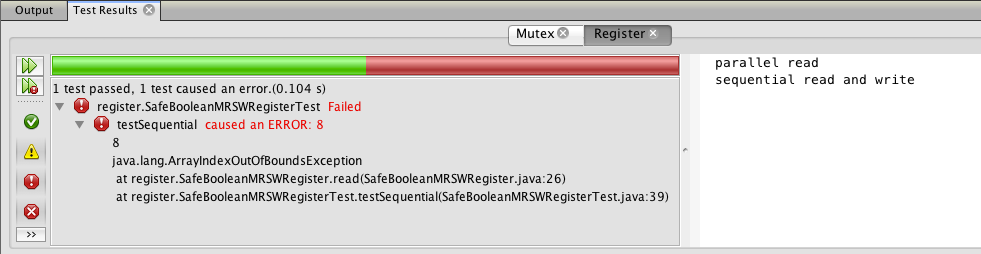
\includegraphics[width=13cm]{SafeBooleanMRSW00.png}
  \caption{First type of failure}
  \label{fig:SafeBooleanMRSW00}
\end{figure}
\par
\begin{figure}[h]
  \centering
  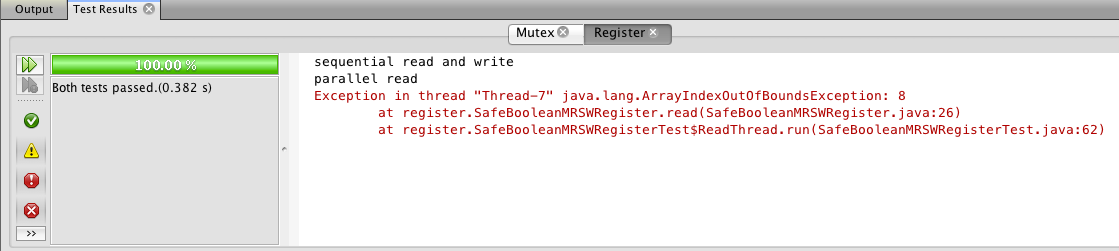
\includegraphics[width=13cm]{SafeBooleanMRSW01.png}
  \caption{Second type of failure}
  \label{fig:SafeBooleanMRSW01}
\end{figure}
\par
So, the way to fix this problem was to make sure that in each test case
the threads ids are reset calling the static method $ThreadID.reset()$. With
this hack, the tests passed (See figure \ref{fig:SafeBooleanMRSW02}).
\par
\begin{figure}[h]
  \centering
  \includegraphics[width=13cm]{SafeBooleanMRSW02.png}
  \caption{Output after fix}
  \label{fig:SafeBooleanMRSW02}
\end{figure}
\par
\begin{figure}[h]
  \centering
  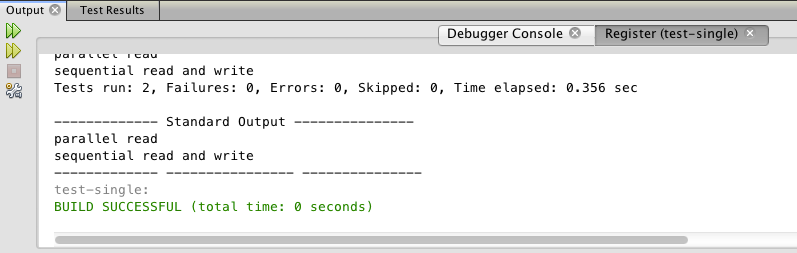
\includegraphics[width=13cm]{SafeBooleanMRSW03.png}
  \caption{Output after fix of threadIds}
  \label{fig:SafeBooleanMRSW03}
\end{figure}
\par
% ------------------------------------------------------------------------------------ %
\subsection{Interpretation}
\par
In this experiment we saw a way of implementing Safe Multi-Reader Single-Writer
registers. These registers were able of storing boolean values.
\par
Unfortunately, none of the test cases excersice the case where we have
concurrent writes and reads. Hence, this experiment only excersiced one of the
two rules of a safe register.
% ------------------------------------------------------------------------------------ %
